\subsection{Implementation}
Our framework is implemented with Pytorch. We used AES-GCM-128 as the authenticated encryption algorithm as Bonawitz \emph{et al}. did~\cite{Practical}. We adopted MNIST and CIFAR-10 as datasets, which are also used in the original FedAvg~\cite{mcmahan2016communicationefficient}. We trained a simple convolutional neural network for the classification task. Our experiments are carried on a PC with an Intel i7-8700 CPU (3.2GHz), 16 GB of RAM, and a GTX 1080 GPU. The model was executed in a single thread to facilitate comparing and analyzing. The optimizer was stochastic gradient descent (SGD) and the learning rate is $0.01$. The $fraction$ is set as $0.1$ which means that $10\%$ of clients will be chosen to carry on the training process in each epoch. 
% Our demo is open-sourced on \url{https://github.com/Carudy/DemoFL}.


\subsection{Accuracy}
Although our work does not modify the learning module compared to other federated learning frameworks, we still conducted a series of experiments to observe the accuracy. We compared FedAvg with our framework on both independently identically distribution (IID) data and non-IID data to verify the effectivity. Since this experiment aims to prove the validity instead of high accuracy, the models were not trained to obtain high accuracy. We conducted experiments with MNIST in non-IID and CIFAR-10 in IID, and Figure~\ref{acc} shows the result. With IID data, our framework obtains a similar performance compared with FedAvg. With non-IID data, the two systems did not match as well as they were with IID data when the $epoch$ was small. However, they finally converged to the same stable scope with the same speed, which confirmed the differences were caused by biases. Therefore, our framework can achieve a same learning goal as FedAvg while providing privacy guarantees and system robustness.

\begin{figure}[!ht]
    \centering
    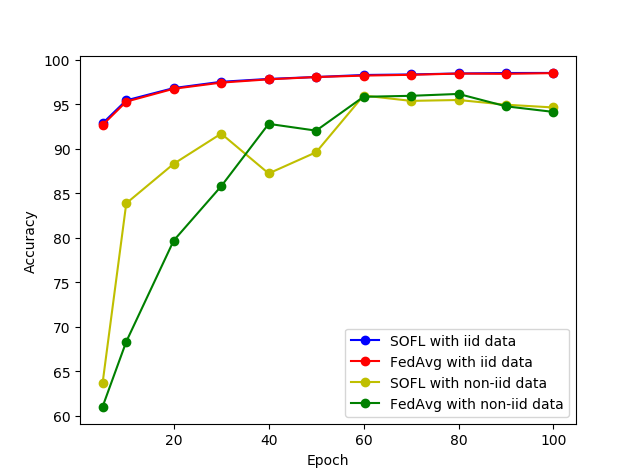
\includegraphics[width=\columnwidth]{img/acc.png}
    \caption{The accuracy of FedAvg~\cite{mcmahan2016communicationefficient} and DemoFL with IID data from CIFAR-10, and non-IID data from MNIST. The horizontal axis $epoch$ means the total rounds that the federated learning system has been trained for. }
    \label{acc}
\end{figure}

\begin{figure}[!ht]
    \centering
    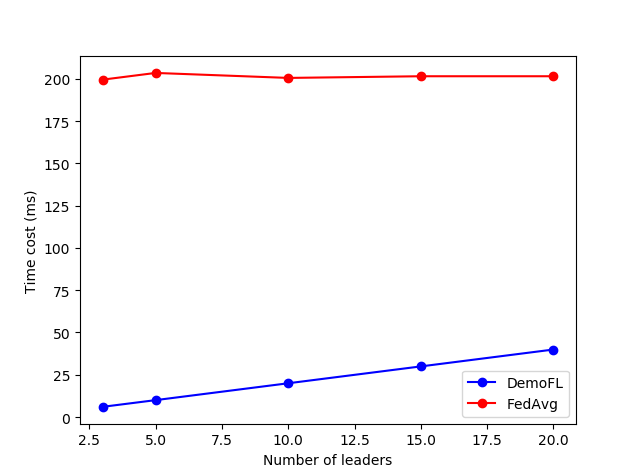
\includegraphics[width=\columnwidth]{img/leader-time.png}
    \caption{The average time spent on computation in set-up process DemoFL VS different proportions of leaders.}
    \label{leader-time}
\end{figure}

\subsection{Set-up Overhead}
In the set-up phase, our system selects several clients as leaders, and the number of leaders impacts the efficiency and a particular leader's load because a common user needs to build secure communication channels with all leaders. To discover the relation between number of leaders and the computaion overhead, we set the number of clients in different levels, and conducted experiments with different number of leaders. Figure~\ref{leader-time} shows the linear relation between each user's computation time spent on Diffie Hellman key-exchange protocol and the number of leaders. The overhead of time in set-up process is also very low because DemoFL has no complex calculations as Bonawitz \emph{et al}.~\cite{Practical}'s secure aggregation scheme does. In Bonawitz's scheme, participants need to calculate secret keys for all other users, and generate t-out-of-n secret shares for the pseudorandom generator (PRG) seed and their secret keys. The comparison is illustrated in Figure~\ref{avg-user-cpu}. Since Bonawitz's scheme has a time complexity of $O(n^2)$, the computation overhead of it is much higher than DemoFL. Method of Kanagavelu \emph{et al}.~\cite{Two-Phase} performs the same as Bonawitz's scheme because they also have an $O(n^2)$ set-up. Therefore, employing fewer leaders can help to improve efficiency, and in contrast, employing more leaders can are beneficial to security because a successful attack requires all leaders compromised. 

Meanwhile, with more leaders, one common user needs to store more keys for leaders. Apparently, the relationship between the number of leaders and one user's storage overhead is also linear. However, in Bonawitz's scheme, a client needs to storge two t-out-of-n secret shares for all others. The storage complexity of DemoFL and Bonawitz's scheme is $O(N_l)$ and $O(n)$ repectively, where $N_l \ll n$. Therefore, DemoFL has a very trivial set-up overhead on both time and storage, which is friendly to individual participants such as smart phones.

\begin{figure}[!ht]
    \centering
    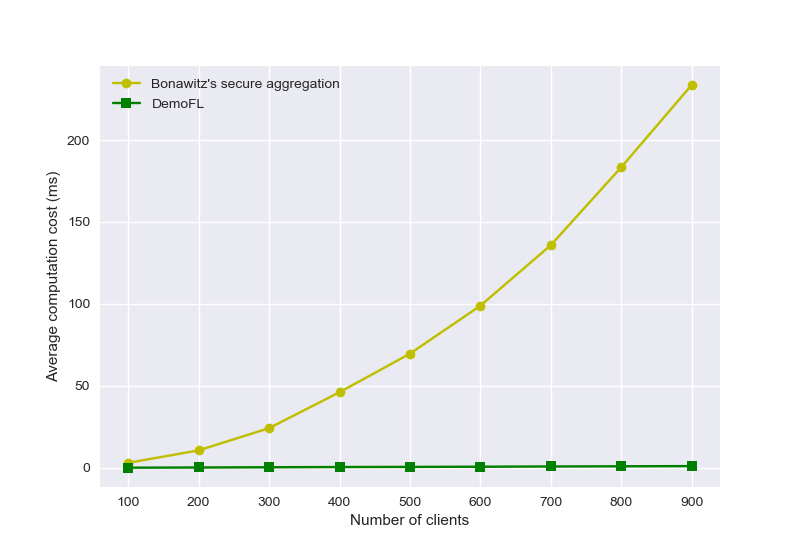
\includegraphics[width=\columnwidth]{img/avg-user-cpu.png}
    \caption{The average time spent on computation in set-up process of Bonawitz's secure aggregation~\cite{Practical} and DemoFL VS the number of clients. The number of leader is 3\% of all participants in DemoFL.}
    \label{avg-user-cpu}
\end{figure}

\subsection{Efficiency}
As introduced before, the overhead of multi-party computation is insignificant compared to the communication overhead in DemoFL. Since the communication cost varies with equipment and environments, it is more sufficient to measure the overhead using the number of communications instead of wall clock time. Note that communication in our simulation means two communications in practice: a user needs to send a message to the server first, and the server forwards the message to the corresponding leader. We fixed the number of leaders to 3. The amount of communications increases with the $epoch$, and the result is displayed in Figure~\ref{comm-epoch} with the assumption that there is no dropout of packets. The number of users is another factor that impacts efficiency. We conducted experiments with the $epoch$ set to 30 and got the results shown in Figure~\ref{comm-client}. The result is the same as what we analyzed in Section IV, which means they are all of the linear time complexity. Although the number of leaders also has an influence on the number of communications, we did not conduct corresponding experiments because it is always set as a very small number. 


\begin{figure}[!ht]
    \centering
    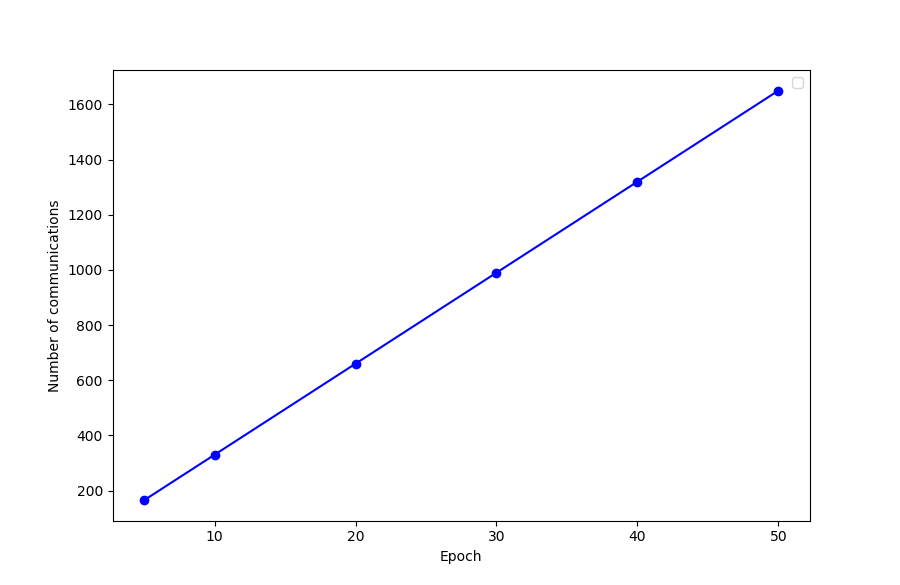
\includegraphics[width=\columnwidth]{img/comm-epoch.png}
    \caption{The amount of communications in learning process with 100 clients without dropout.}
    \label{comm-epoch}
\end{figure}

\begin{figure}[!ht]
    \centering
    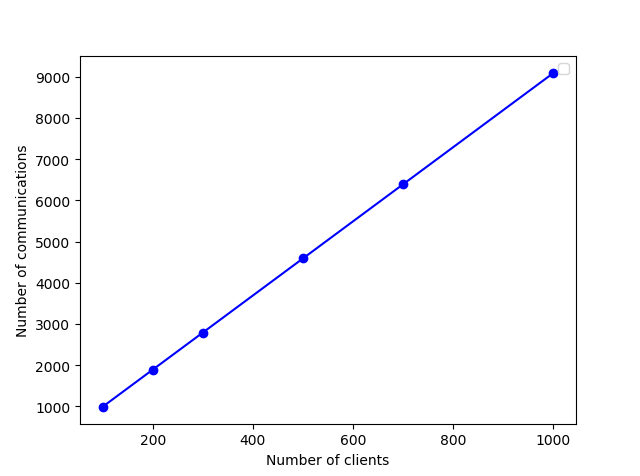
\includegraphics[width=\columnwidth]{img/comm-client.png}
    \caption{The amount of communications in learning process varies VS  the amount of clients. The $Epoch_{max}$ is fixed to 30 and there is no dropout.}
    \label{comm-client}
\end{figure}


\subsection{Robustness}
\subsubsection{Crash}
The robustness of DemoFL is mainly based on the re-organizing process, which happens when a leader is crashed. Crashes can hardly be completely avoided, therefore, we introduced $crash\_rate$, which is the possibility that a leader would crash during one epoch, to help to measure the robustness. Generally, we consider $crash\_rate$ is quite small because real crashes rarely happen in nowadays smart devices/servers. However, compared to real crashes, a leader is more likely to be unavailable due to various reasons, which also seldom happens. Therefore we can consider $crash\_rate$ would not be larger than $0.1$. We conducted several experiments on how $crash\_rate$ impacts efficiency. First, we set the number of clients to 100 and the $Epoch_{max}$ to 10. Figure~\ref{comm-crash} shows that when crashes happened, it impacts the same on the value of communications instead of the ratio despite the $epoch$. E.g., a crash with $epoch$ 10 resulted in $66\%$ overhead approximately, and it only resulted in about $0.06\%$ overhead when the $epoch$ is $100$. It indicates that a high $crash\_rate$ does impact the efficiency heavily when $epoch$ is low. However, when the $epoch$ gets larger, the influence of crashes becomes insignificant. Considering that the $epoch$s used in real federated learning works are quite large, DemoFL provides sufficient efficiency and robustness.

\begin{figure}[!ht]
    \centering
    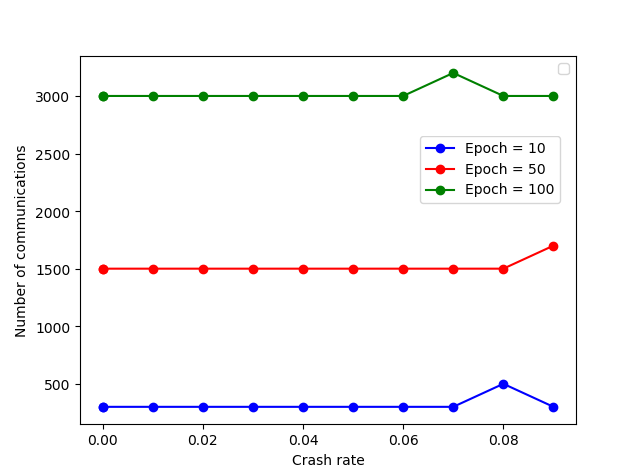
\includegraphics[width=\columnwidth]{img/comm-crash.png}
    \caption{The average amount of communications VS different crash rates.}
    \label{comm-crash}
\end{figure}

\begin{figure}[!ht]
    \centering
    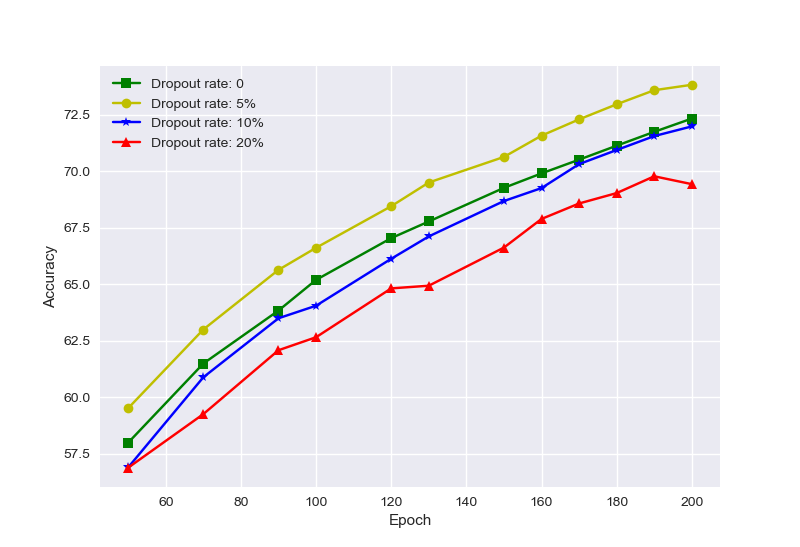
\includegraphics[width=\columnwidth]{img/dropout-acc.png}
    \caption{The accuracy VS different dropout rates.}
    \label{dropout-acc}
\end{figure}

\subsubsection{Network Delay and Dropout}
Sometimes several packets cannot be received in time due to network delays or dropouts. Bonawitz \emph{et al}.'s method~\cite{Practical} has considered this issue and it has a pseudorandom generator (PRG) based masking algorithm to solve it, which has a high computation overhead. In DemoFL's secure learning process, a leader will not be waiting for participants'parameters permanently. It has a time limit, over which the leader will abandon waiting and send the current $B_j$ to the server (introduced in Section~\ref{sec:DemoFL}). Under this circumstance, some common parties will be recognized as having lost connection and removed from the participant-group without contributing to the learning process. However, if a party does not lose the connection while its message reached the leader late because of network delay, discarding it may influence the learning speed and result. We set the dropout rate to show the probability that a common party fails to send its parameters to leaders due to packet loss or network delay. Therefore, we carried out several experiments to observe how network delay impacts the learning process. The result is shown in Figure~\ref{dropout-acc}. We observed that the influence of dropouts on accuracy becomes trivial as the learning process goes on. The accuracy is reduced by only 0.002 in the worst case, which may be caused by biases. Therefore, DemoFL has a strong resistance to packet loss. 